\newpage
\section{Comparative Analysis}

\subsection{Introduction}

In this section, we conduct a comparative analysis between ChatGPT and Google Bard on the \textbf{reliability} and \textbf{privacy} aspects. By reliability, we are referring to how well the system might function for people across different use conditions and contexts, including ones it was not originally intended for. And more broadly, how accurate and relevant the model responses are. The privacy aspects include data breach issues, unauthorised use of private data and unclear sources of training data. Both models were released in the same time period, ChatGPT-3.5 was released on November 30, 2022 while Google Bard was publicly available on March 21, 2023. As two of the most prominent and continuously evolving chatbots, their popularity and relatively similar timelines make Bard a good target to be compared with. Next, we examine more recent technologies to assess whether these issues have been addressed or persist to this day.

The \textbf{focus} of this comparative analysis is \textbf{incompleteness and flaws} of the two LLMs in reliability and privacy aspects, however, \textbf{we should not overlook the advantages} of these two AI chatbots. A study by \cite{laskar2023systematic} evaluated ChatGPT on 140 diverse NLP tasks and showed its impressive performance in several benchmarks dataset. Though it does not surpass fine-tuned models in specific fields, it confirms ChatGPT-3.5's general capacity as a pre-trained LLM. The study also pointed out ChatGPT possess human-level problem solving skills and its strength at math and coding. The strong general performance of ChatGPT-3.5 can be further leveraged to a fine-tuned model using \textbf{reinforcement learning from human feedback (RLHF)}. \cite{ouyang2022training} showed that fine-tuning GPT model significantly improves the performance on different tasks. Similarly for Google Bard, from the original paper released by Google (\cite{thoppilan2022lamda}), large data size used to train LaMDA contributes to more sensible, specific and interesting responses compared to smaller models.

The following discussions under this section are inspired by prior analyses, which provides a comprehensive overview of the comparison between ChatGPT and Google Bard (\cite{Ahmed2024}).

\subsection{Model Background}

Both chatbots are pre-trained on a vast amount of data, combining with transformer architecture and reinforcement learning techniques. This allows the model to process long and complex queries and generate the next word based on the previous texts.

While OpenAI didn't reveal the exact amount of parameters used in the GPT-3.5 model, they did reveal (\cite{Brown2020}) that around 175 billion parameters have been used for GPT-3, which is the base of GPT-3.5. On the other hand, the very first version of Google Bard which was based on LaMDA (Language Models for Dialog Applications) and had 137 billion parameters and the size of the dataset for pretraining is 1.56 trillion words (\cite{Thoppilan2022}). A key distinction between these two models is that Bard had real-time web access. This enabled Bard to retrieve the newest data from the internet while ChatGPT is trained on fixed, historical dataset and lacked flexibility to adapt to new changes.

\subsection{Reliability}

Even though the LLMs like ChatGPT and Bard are powered with vast amount of parameters and large dataset for pretraining, they still suffer from \textbf{``Artificial Hallucinations''}, where the AI generates seemingly reasonable texts but do not correspond to the actual input (\cite{Alkaissi2023}). A systematic review (\cite{Chelli2024}) was conducted to compare the hallucination rates between GPT-3.5, GPT-4 and Bard. For the scope of this report, we only focus on the comparison between GPT-3.5 and Bard. The study selectively picks 11 systematic reviews from different medical fields and prompts LLMs with the same inclusion criteria as human-conducted systematic reviews. Finally compare the references generated by LLMs with original systematic review references. The aim of the study is to assess the performance of LLMs to generate references for academic use.

\begin{figure}[h]
    \centering
    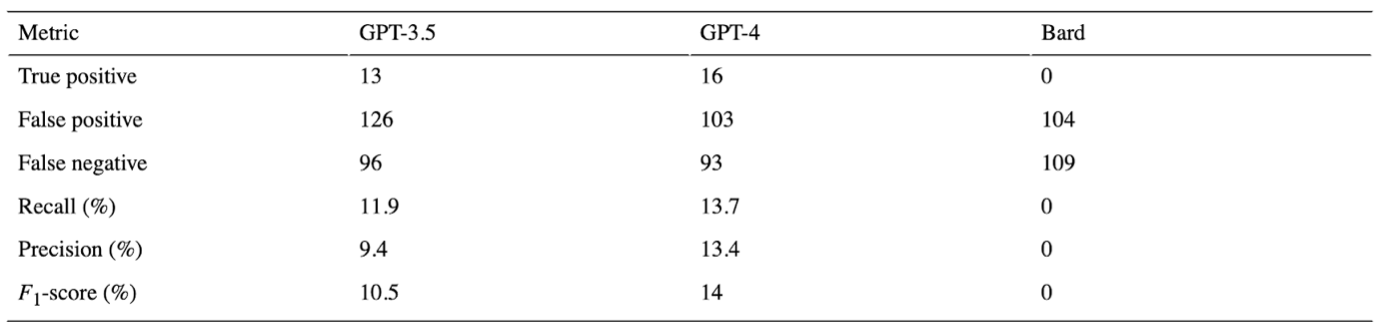
\includegraphics[width=0.8\textwidth]{image2.png}
    \caption{Comparison of systematic review performance between GPT-3.5 and Bard}
    \label{fig:image2}
\end{figure}

The table from the study demonstrates the final evaluative metrics. Bard failed to retrieve any paper from the systematic reviews while GPT-3.5 successfully retrieved some.

Note that in this study, Bard is based on PaLM2, which is an upgraded version evolved from LaMDA and then PaLM before reaching PaLM2. The fact that GPT-3.5 still outperforms Bard in multiple metrics demonstrates that ChatGPT was already significantly superior to Bard by the time Bard was first released. Despite the integration with Google search, Bard still faces significant challenges in complex tasks. At the time of analysis, Bard's AI was still in the developing phase and exhibited more errors and hallucinations, while ChatGPT offered a more accurate model in general.

% Privacy Section for the Comparative Analysis

\subsection{Privacy}

Back to 2023, there were several articles stating their privacy concerns that users' private data may get leaked through ChatGPT and showed the tricks to do so. \cite{NYT2023ChatGPTPrivacyExploit} explains how a group of researchers in Indiana University extracted his email address from ChatGPT. The researchers were working on a fine-tuned version of GPT-3.5 Turbo and accidentally found that OpenAI did not have the protections on the fine-tuned data, which means requests that would be denied in typical ChatGPT interface may be accepted. In the experiment, the researchers fed ChatGPT with a short list of verified names and email addresses of New York Times employees which caused the model to produce similar results. Though the results suffered from hallucination, 80\% of the email addresses produced were correct. The spokesman from OpenAI claimed that the model did not store or copy the sensitive data in a database. However, LLMs would still look for the relevant data that it has been trained on even if the data were not supposed to be recalled. \cite{Grad2023} also reports that simple commands can be used to retrieve private information in GPT-3.5 Turbo. With \$200 worth of queries, the researchers were able to extract 10,000 unique verbatim memorized training examples (\cite{Nasr2023}). For example, the researchers would request ChatGPT to repeat a certain word endlessly which caused the model to go beyond its training process and fall into a malfunction. Google Bard also faces similar privacy issues regarding the use of Gmail data. \cite{Hanna2023} highlighted this issue in a blog post. Although Google claims that Bard is not trained on any information from Gmail or any private data from other apps, ironically Bard itself says it is trained on Gmail. Since Google never reveals the source of training data, it remains unclear for users whether their private information gets used in the training procedure.

According to the report by \cite{Pietro2023}, ChatGPT had a data breach issue in March 2023, where the model exposed other users' chat histories and even payment information to unintended users. The Italian data regulator chose to temporarily ban ChatGPT because of this incident. While Bard did not have similar data breach issues, it had an incident where the conversation with Bard showed up in public search (\cite{Pieter2023}). This means users' chat may be scraped by Google's scrawler. Google later clarified that only shared links were indexed, but this incident revealed the risk of data exposure when sharing the chat with others.

\subsection{Industry Responses}

Moving onto the end of 2023, the Google Gemini, which is basically rebranded from previous Bard made significant improvement across different domains such as STEM, humanities, general reasoning abilities, math, coding etc (\cite{Pichai2023}). As for the privacy aspect, from the official AI principles published by Google in 2023, a lot of technical techniques were introduced to boost the security of the AI model. Adversarial testing, privacy preserving algorithms, built-in model mitigations etc. were utilised in the AI developing process. OpenAI is also dedicated to resolving privacy issues. The company undergoes regular third-party penetration testing and receives recognition from security standards such as SOC 2 Type2 (Service Organization Control) and CSA STAR Level 1 (Cloud Security Alliance Security Trust Assurance and Risk).

\subsection{Conclusion}

While the performance and reliability of LLMs such as ChatGPT-3.5 and Google Bard based on LaMDA vary across different domains, their overall capabilities represent a significant advancement in NLP. However, we can see that LLMs suffer from hallucination and are bottlenecked by the nature of machine learning. As for the privacy aspect, even though we can observe some improvements in technical and regulatory approach, privacy concerns still persist to this day.

% Word Count: 1349
